%  Created by Alexis on 2012-11-04.
%  Copyright (c) 2012 . All rights reserved.
%
%\documentclass[]{article}
%\documentclass[12pt,pdftex,twocolumn]{article}
\documentclass[12pt,pdftex]{article}
% Use utf-8 encoding for foreign characters
\usepackage[utf8]{inputenc}
% Setup for fullpage use
\usepackage{fullpage}
% Surround parts of graphics with box
\usepackage{boxedminipage}
% Package for including code in the document
\usepackage{listings}
% If you want to generate a toc for each chapter (use with book)
%\usepackage{minitoc}
% This is now the recommended way for checking for PDFLaTeX:
\usepackage{ifpdf}

\ifpdf
\usepackage[pdftex]{graphicx}
\else
\usepackage{graphicx}
\fi

\title{CS760 \\ All In \\ Project Report }
\author{  Alexis Fisher }
%\date{2012-11-04}
\begin{document}
\ifpdf
\DeclareGraphicsExtensions{.pdf, .jpg, .tif}
\else
\DeclareGraphicsExtensions{.eps, .jpg}
\fi
\maketitle
\begin{abstract}
\emph{All In} is a five card draw poker player.  
The implemented player uses reinforcement learning to outperform a random player. 
The learner has imperfect knowledge of the opposing player.
The implemented learner performs better than the random player, winning more than 60\% of games played.

%Intro approach evaluation discussion conclusion
\end{abstract}
\section{Introduction}
%Introduction: what you attempted to do, and what the motivation is.
\emph{All In} implements a 5-card draw poker player. 
The primary goal of the \emph{All In} player is to outperform a random player. 
Initial implementation assumes two players. 
The players consist of the learned player and another player. 
The other player can be either a random actor, a person, or another learned player. 
This paper discusses the approach taken in Section \ref{sec:approach}, presents experimental results in Section \ref{sec:eval}, Section \ref{sec:disc} discusses these experimental results, current limitations, and future work, Section \ref{sec:related} describes a selection of related work, and we conclude in Section \ref{sec:conclusion}.

\section{Approach} \label{sec:approach}
\begin{table*}[ht]
\centering
	\begin{tabular}{| r | r | l |}
\hline
\textbf{Value} & \textbf{Name} & \textbf{Description} \\
\hline
0 & high card & No other match \\
1 & one pair & Single pair of a single value\\
2 & two pairs & Two pairs of distinct values\\
3 & three of a kind & Three cards of a single value\\
4 & straight & Sequentially numbered cards\\
5 & flush & All cards of a single suit\\
6 & full house & Distinct three of a kind and pair\\
7 & four of a kind & Four cards of a single value\\
8 & straight flush & Sequential numbered cards of a single suit\\
9 & royal flush & Straight flush with an Ace as high card\\
\hline
\end{tabular}
\caption{Description of Values according to hand}
\label{tab:cardvalues}
\end{table*}

\emph{All In} uses nondeterministic \emph{Q} reinforcement learning, with a value function determined by the hand's rank and past performance (Wins or Losses). This valuation is described in Table \ref{tab:cardvalues}. 
Because results of a given hand and each given draw are nondeterministic, exploration happens organically. 
Win/Loss probability uses Laplace smoothing to account for values the learner has not yet encountered. This valuation is pessimistic. 
If the learner achieves a royal flush, there is a much higher likelihood of winning than the 50\% indicated in Table \ref{tab:rand_val_res}. 

As the rules of poker can vary widely, a quick description of the ruleset implemented is appropriate.
Each player is dealt a hand of five cards from a standard 52 card deck. 
Each player has the opportunity to discard up to three cards, and receive replacements from the deck.
Poker hands, as described in Table \ref{tab:cardvalues}, are used to determine the winner.

\section{Evaluation} \label{sec:eval}

\subsection{Random Players}
Two random-acting players initially played against each other to gather baseline accuracy information and to provide initial win frequencies to our learner. 
Table \ref{tab:rand_res} shows the win counts of each random player. 
As anticipated, random players approach near-even wins and losses.
Table \ref{tab:rand_val_res} shows a breakdown of the observed behavior for a single learner. 
Values that were not seen in the 40,000 games have a win likelihood of 50\% due to smoothing.
These tables show the range of observed behaviors and expected outcomes after approximately 40,000 games.
Figure \ref{fig:rand_v_rand} shows the performance of a single random player, playing against another random player, over a series of distinct games.  We expect this to oscillate around 50\% wins. 

\begin{table}[h]
\centering
\begin{tabular}{| l | c | c |}
	\hline
& \textbf{Random 1} & \textbf{Random 2}\\
\hline
Wins & 18963 & 21461\\ %Total: 40424
	\hline
Win Percentage & 47\% &53\% \\
\hline
\end{tabular}
\caption{Game Results with Random Players}
\label{tab:rand_res}
\end{table}

\begin{figure}[hb!]
	\begin{center}
		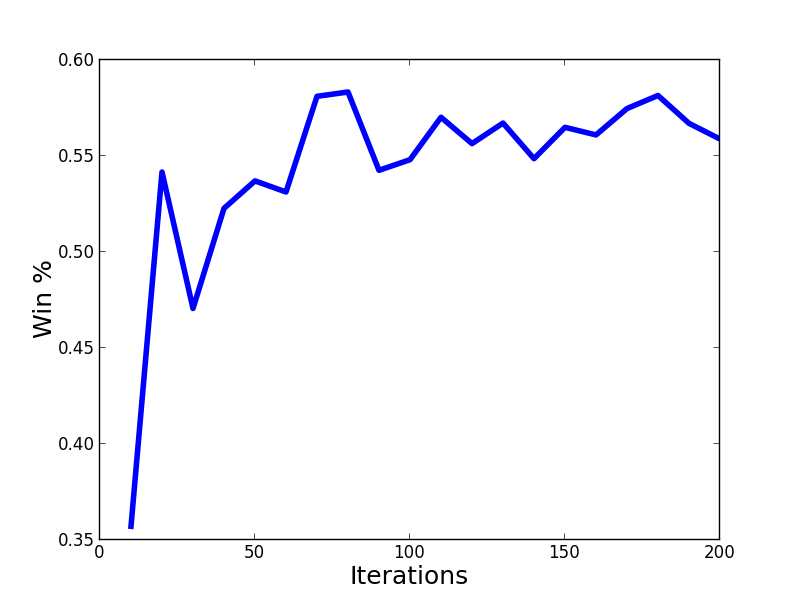
\includegraphics[scale=0.5]{figs/randvrand.png}
		\caption{Random Wins vs. Random}
		\label{fig:rand_v_rand}
\end{center}
\end{figure}

\begin{table*}[ht!]
\centering
\begin{tabular}{| l | r | l | r | l |}
	\hline
 \textbf{Value} & \textbf{Wins}& \textbf{Losses}& \textbf{Total}& \textbf{Expected Win \%}\\
\hline
0& 8823& 11484& 20307& 43.4487173174\\
1& 10400& 6708& 17108& 60.7890122735\\
2& 1424& 498& 1922& 74.0644490644\\
3& 647& 168& 815& 79.3145654835\\
4& 87& 72& 159& 54.6583850932\\
5& 46& 28& 74& 61.8421052632\\
6& 27& 3& 30& 87.5\\
7& 7& 2& 9& 72.7272727273\\
8& 0& 0& 0& 50.0\\
9& 0& 0& 0& 50.0\\
\hline
\end{tabular}
\caption{Expected Game Results with Random Players by Value}
\label{tab:rand_val_res}
\end{table*}

%%%%%%%%%
\subsection{Learner vs. Random Player}
\begin{table*}[h]
\centering
\begin{tabular}{| l | r | l | r | l |}
	\hline
 \textbf{Value} & \textbf{Wins}& \textbf{Losses}& \textbf{Total}& \textbf{Expected Win \%}\\
\hline
0& 148& 153& 301& 49.1749174917\\
1& 195& 66& 261& 74.5247148289\\
2& 22& 1& 23& 92.0\\
3& 9& 0& 9& 90.9090909091\\
4& 0& 0& 0& 50.0\\
5& 4& 0& 4& 83.3333333333\\
6& 2& 0& 2& 75.0\\
7& 0& 0& 0& 50.0\\
8& 0& 0& 0& 50.0\\
9& 0& 0& 0& 50.0\\
\hline
\end{tabular}
\caption{Expected Game Results, Learner vs. Random Player from Learner's Perspective}
\label{tab:learner_v_rand}
\end{table*}
\begin{figure}[h]
	\begin{center}
		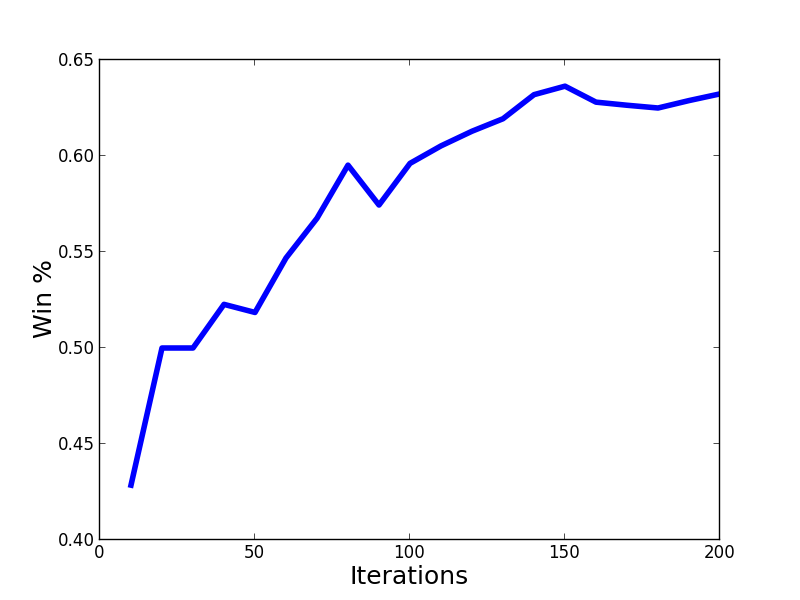
\includegraphics[scale=0.5]{figs/learnervrand.png}
		\caption{Learner Wins vs. Random}
		\label{fig:learner_v_rand}
\end{center}
\end{figure}

The learner played against a random player to ascertain performance improvement in our learner over random actions. 
This performance improvement is evident in Table \ref{tab:learner_v_rand}. 
The learner, primed with the results from the random players, won 63\% of the time.  
The learner's win after different amounts of iterations is demonstrated in Figure \ref{fig:learner_v_rand}.
Figure \ref{fig:learner_v_rand} shows performance improvement as more results are gathered and incorporated into the learner's model.

%%%%%%%%%%%
\subsection{Learner vs. Learner with background}
The learner also played against another instance of our learner, each with identical background information.
This background information included the body of results from the random players, as well as the body of results from the learner versus the random player. 
The winning percentages over a range of iterations is shown in Figure \ref{fig:learn_v_learn}.
These are approximately even, as expected. 

\begin{table*}[hb!]
\centering
\begin{tabular}{| l | r | l | r | l |}
	\hline
 \textbf{Value} & \textbf{Wins}& \textbf{Losses}& \textbf{Total}& \textbf{Expected Win \%}\\
\hline
0& 26& 36& 62& 40.625\\
1& 35& 22& 57& 59.3220338983\\
2& 8& 0& 8& 80.0\\
3& 3& 0& 3& 60.0\\
4& 0& 0& 0& 0.0\\
5& 0& 0& 0& 0.0\\
6& 1& 0& 1& 33.3333333333\\
7& 0& 0& 0& 0.0\\
8& 0& 0& 0& 0.0\\
9& 0& 0& 0& 0.0\\
\hline
\end{tabular}
\caption{Expected Game Results, Learner1 vs. Learner2 from Learner1's perspective}
\label{tab:learner1_v_learner}
\end{table*}

\begin{table*}[hb!]
\centering
\begin{tabular}{| l | r | l | r | l |}
	\hline
 \textbf{Value} & \textbf{Wins}& \textbf{Losses}& \textbf{Total}& \textbf{Expected Win \%}\\
\hline
0& 24& 48& 72& 32.4324324324\\
1& 25& 24& 49& 49.0196078431\\
2& 5& 0& 5& 71.4285714286\\
3& 4& 1& 5& 57.1428571429\\
4& 0& 0& 0& 0.0\\
5& 0& 0& 0& 0.0\\
6& 0& 0& 0& 0.0\\
7& 0& 0& 0& 0.0\\
8& 0& 0& 0& 0.0\\
9& 0& 0& 0& 0.0\\
\hline
\end{tabular}
\caption{Expected Game Results, Learner1 vs. Learner2 from Learner2's perspective}
\label{tab:learner2_v_learner}
\end{table*}

\begin{figure}[ht!]
	\begin{center}
		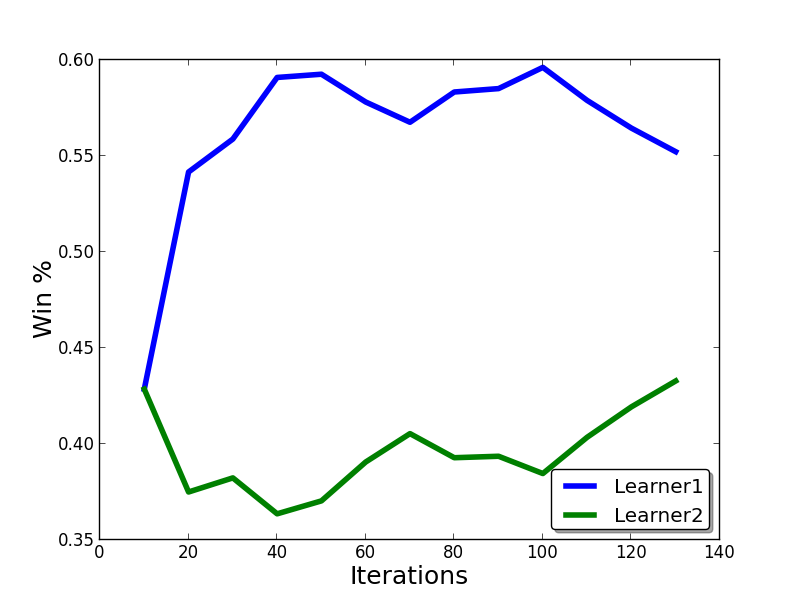
\includegraphics[scale=0.5]{figs/learnervlearner.png}
		\caption{Learner Wins vs. Learner}
		\label{fig:learn_v_learn}
\end{center}
\end{figure}

%%%%%%%%%%%
\subsection{Learner vs. Learner without background}
The learner, starting with no background information, played another instance of the learner with no background information.
Figure \ref{fig:learn_v_learn_hist} shows the win ratio after a range of game iterations.
As expected, both instances of the learner, although they each have distinct information, oscillate around 50\% win ratios.

\begin{figure}[ht!]
	\begin{center}
		\includegraphics[scale=0.5]{figs/learnervlearner_hist.png}
		\caption{Learner Wins vs. Learner}
		\label{fig:learn_v_learn_hist}
\end{center}
\end{figure}

%%%%%%
%TODO
%\subsection{Learner with background vs. Learner without background}
%The learner with background information of only learner's performance (omitting the information from plays of only random players) played against another instance of the learner with no background information.

\section{Discussion} \label{sec:disc}
\subsection{Results}
Results show the learner performs better than the random actor. 
When the learner plays against itself, each instance of the learner appears to win about 50\% of the time.

\subsection{Limitations}
\label{subsec:limit}
The value function currently only takes hand rank into account, not card value within rank. A hand consisting of ``2 of Clubs, 3 of Hearts, 7 of Diamonds, Jack of Spades, Ace of Hearts'' is equivalent to a hand consisting of ``2 of Hearts, 3 of Hearts, 7 of Diamonds, 8 of Spades, Jack of Hearts'' -- both are currently valued as ``high card'' hands, with no extra weight given to the ace-high hand. 
If these hands are played against each other, the ace-high hand will win and the jack-high hand will lose, but our learner does not take into account actual hand values seen in its predictive function.

\subsection{Future Work}
Future work could include incorporating wagers into \emph{All In}.  
Accounting for wagers is a much richer environment, and was outside the scope of this project.  
This would also require the possibility folding after the initial wager and deal, as well as tracking funds over a series of hands.

Incorporating specific hands, as described in Subsection \ref{subsec:limit}, could provide for further gains in performance.
This does run the risk of requiring more smoothing, as the incorporated data would be sparser.
This could be ameliorated by falling back to a simple value estimation if no hand estimation exists, or by weighting the smoothing applied by value (i.e., 90\% probability to win if the hand is a royal flush, 80\% probability to win if the hand is a straight flush, etc.).

If the learner incorporated how many cards are chosen to swap with wins and losses, this may garner more insight into results.
It's undetermined if there would be useful gains, but might be an interesting avenue to explore.

\section{Related Work} \label{sec:related}
There are many discussions of reinforcement learning and games, especially poker and its variants.
There does not seem to be any work on this particular variant of poker, five card draw.  

Erev et al.\ explore a variety of games, and show that their reinforcement model outperforms equilibrium predictions \cite{Erev98}.  

Dahl applies a reinforcement learning algorithm to two-layer Texas Hold'em Poker \cite{Dahl01}. 
This differs from our use of five card draw as a game, and changes the amount of information available about the other agent's status. 

Sweeney et al.\ explores the use of reinforcement learning to Texas Hold'em Poker \cite{Sweeney}.
This again differs from our use of five card draw as the game of choice.  
Wagering information and past actions of the opponent are taken into consideration in the described learning model.

\section{Conclusion} \label{sec:conclusion}
\emph{All In} implements a 5-card draw poker player. 
The primary goal of the \emph{All In} player is to outperform a random player. 
%Initial implementation assumes two players. 
The players consist of the learned player and another player. 
The other player can be either a random actor, a person, or another learned player. 
The reinforcement \emph{All In} learner is shown to perform better than a random player.
A selection of related works are also presented.
%Source code is available at

\bibliographystyle{plain}

\begin{thebibliography}{9}
\bibitem{korb99}
K.B. Korb, A.E. Nicholson and N. Jitnah,
 \emph{Bayesian Poker}. 
In Proc. of Uncertainty in Artificial Intelligence, pp. 343-350, 
Stockholm, Sweden, August, 1999.

%\bibitem{pokerdata}
%\emph{Poker Hand Data Set}
%http://archive.ics.uci.edu/ml/datasets/Poker+Hand

\bibitem{Sweeney}
Neill Sweeney, David Sinclair,
	\emph{Applying Reinforcement Learning to Poker}.
At Computer Poker Symposium, July, 2012.

\bibitem{Erev98}
Ido Erev and  Alvin E Roth, 
\emph{Predicting How People Play Games: Reinforcement Learning in Experimental Games with Unique, Mixed Strategy Equilibria}.
In American Economic Review, American Economic Association, vol. 88(4), pages 848-81, September, 1998.

\bibitem{Dahl01}
Fredrik A. Dahl, 
\emph{A Reinforcement Learning Algorithm Applied to Simplified Two-Player Texas Hold'em Poker}. 
In Proceedings of the 12th European Conference on Machine Learning (EMCL '01), Luc De Raedt and Peter A. Flach (Eds.). Springer-Verlag, London, UK, UK, 85-96, 2001.
\end{thebibliography}


\end{document}
